\documentclass{ximera}

\title{Sample interactives}
\author{Jim Fowler}

\begin{document}
\begin{abstract}
Testing interactives and ff.
\end{abstract}
\maketitle

\begin{javascript}
  window.isPositive = function(number) {
    return number > 0;
  };

  window.sameParity = function(a,b) {
    return (a-b)%2 == 0;
  };

  window.caseInsensitive = function(a,b) {
    return a.toLowerCase() == b.toLowerCase();
  };
\end{javascript}

\begin{problem}
  Pick an integer larger than 10, like $\answer[format=integer,validator=this>10]{11}$.

  Pick $\answer[format=integer,validator=isPositive]{17} > 0$.

  Find a solution to $\answer[format=integer,validator=sameParity]{5} \equiv 5 \bmod 2$.

  String equality is like $\mbox{Word} = \answer[format=string]{Word}$, but $\mbox{Word} = \answer[format=string,validator=caseInsensitive]{Word}$ is good too.
\end{problem}

%%%%%%%%%%%%%%%%
%%%%%%%%%%%%%%%%
%%%%%%%%%%%%%%%%
%%%%%%%%%%%%%%%%

\begin{sagesilent}
  x = var('x')
  a = 17
  b = 12
  c = 10
  f = a*x*x + b*x + c

  kind = 'saddle'
\end{sagesilent}

The polynomial is $\answer{\sage{f}}$.


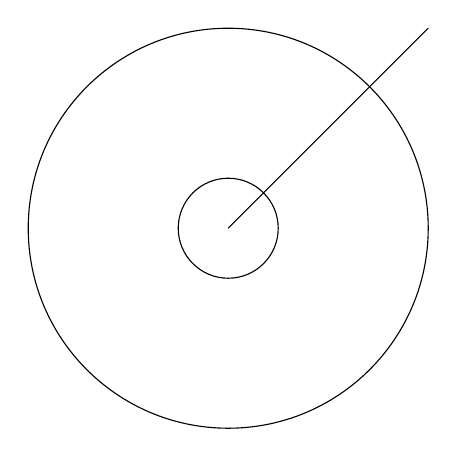
\begin{tikzpicture}
  \draw (0,0) circle (1in);
  \draw (0,0) circle (0.25in);
  \draw (0,0) -- (1in,1in);
\end{tikzpicture}

\begin{problem}


  So pick a variable.
  \begin{multipleChoice}[id=v]
    \choice[correct,value=x]{$x$}
    \choice[value=y]{$y$}
    \choice[value=z]{$z$}
  \end{multipleChoice}

  % propagate right and wrong to other \js places
  You picked $\js{v}$ or, in text, \js{v}.

  %\begin{javascript}
  %  bob.on('change', function() {
  %    px = bob.x;
  %    py = bob.y;
  %  });
  %\end{javascript}

  %$(\answer[id=px,format=float]{4},\answer[id=py,format=float]{4})$

  $\answer[id=n,format=integer]{3}$

  \begin{javascript}
    bob.n_e = n;
  \end{javascript}
  
  \begin{validator}[bob.n_e == 3]
  %  \includeinteractive[id=bob,x=px,y=py]{example2.js}
  
    \includeinteractive[id=bob,width=10,height=10]{phase.js}

  %  $(\js{bob.x},\js{bob.y})$
  \end{validator}

  You used \js{bob.n_e} points.

\end{problem}

\begin{problem}
  Find two integers which sum to twenty five.

  % this should be a callback potentially (I guess if it returns a function?)
  \begin{validator}[a+b==25]
    $\answer[format=integer,id=a]{16} + \answer[format=integer,id=b]{9} = 25$.
  \end{validator}

  Find a traceless matrix with integer entries.
  \begin{validator}[a11+a22==0]
    \[
      \begin{bmatrix}
        \answer[format=integer,id=a11]{0} &         \answer[format=integer,id=a12]{0} \\
        \answer[format=integer,id=a21]{0} &         \answer[format=integer,id=a22]{0} \\
      \end{bmatrix}
      \]
  \end{validator}


\end{problem}

\begin{problem}
  Or just $\answer[format=string]{WHEE}$.

  So the format determines a default validator, like format=string determines validator=stringEquality.  And now I removed the CDATA.
\end{problem}


\begin{problem}
  %An example of a positive number is $\answer[id=z,validator=isPositive(z)]{17}$.

  %$\answer[validator=this>0]{17}$.

  % validator should return 0 or false, 1 or true, partial credit btween 0 and 1, ...
  %$\answer[validator=isPositive]{17}$.

  The tolerance (0.01) means $8 \approx \answer[tolerance=0.01,id=x,format=integer]{8}$
  
  \begin{feedback}
    The answer is definitely more than five.
  \end{feedback}

  \begin{feedback}[x==10]
    The answer is certainly not ten.
  \end{feedback}

  A function is $f(x) = \answer[id=f]{x^2}$.
\end{problem}

\begin{javascript}
  letters = word.length;
\end{javascript}

And another one.  $x + 10 = \js{x+10}$ is equal to \js{x + 10}.

Since $f(\js{v}) = \js{f}$, we decide what?  Well then $f'(\js{v}) = \js{f.derivative(v)}$.

And the word ``\js{word}'' is \js{letters} letters long.

$\js{2+5} = 7$.

\end{document}
